\documentclass{beamer}
\usetheme{Warsaw}

\usepackage[utf8]{inputenc}
\usepackage{fancybox}
\usepackage{multimedia} 
\usepackage{subfig}
\usepackage{amsmath}
\usepackage{hyperref}
\usepackage{marvosym}

\usepackage[all]{xy}
\begin{document}


\title[Digitale Bildverarbeitung] % (optional, only for long titles)
{Digitale Bildverarbeitung
\\
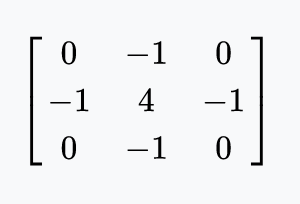
\includegraphics[scale=1.0]{img/cover}
}
\subtitle{}
\author[Dr. Johannes Riesterer] % (optional, for multiple authors)
{Dr.  rer. nat. Johannes Riesterer}

\date[KPT 2004] % (optional)
{}

\subject{Digitale Bildverarbeitung}

\frame{\titlepage}


\begin{frame}
    \frametitle{Frequenz- und Skalenraummethoden}
\framesubtitle{}

\begin{block}{Fourier-Reihe}
Für eine $2\pi$ periodische Funktion $f: \mathbb{R} \to \mathbb{C}$  heißt 
\begin{align*}
Sf_n(x) := \sum_{k= -n}^{n} \hat{f}(k) \cdot e^{ikx} 
\end{align*}
die Fourier-Reihe von $f$ vom Grad $n$ mit den den Fourier-Koeffizienten
\begin{align*}
\hat{f}(k) := \frac{1}{2 \pi} \int_{[0, 2 \pi]} f(t) \cdot e^{-ikt} \; dt
\end{align*}
\end{block}

 \end{frame}


\begin{frame}
    \frametitle{Frequenz- und Skalenraummethoden}
\framesubtitle{}

\begin{block}{Fourier-Reihe}
Ist $f$  $2\pi$-periodisch,  stetig und stückweise stetig differenzierbar, so konvergiert die Fourierreihe gleichmässig gegen $f$, es gilt dann also 
\begin{align*}
\lim_{n \to \infty} \max_x |Sf_n(x) -f(x) | = 0
\end{align*}
\end{block}

 \end{frame}



\begin{frame}
    \frametitle{Frequenz- und Skalenraummethoden}
\framesubtitle{}

\begin{block}{Fourier-Reihe - Interpretation}
Es ist $e^{-ikt} := \cos (k t) + i \sin(kt)$ und 
\begin{align*}
  \frac{1}{2 \pi}  \int_{[0, 2 \pi]}  e^{-ilt} \cdot e^{-ikt} \; dt = \begin{cases} 1 \text{ für k = l}  \\ 0 \text{ sonst }\end{cases}
\end{align*}
Die Funktionen  $e^{-ikt}$ bilden bezüglich des Skalarproduktes $\langle f, g \rangle : =\frac{1}{2 \pi}  \int_{[0, 2 \pi]}  f(t) \cdot g(t) \; dt$ eine orthonormalbasis der $2\pi$-periodisch, stetig und stückweise stetig differenzierbaren Funktionen.
\end{block}
 \end{frame}


\begin{frame}
    \frametitle{Frequenz- und Skalenraummethoden}
\framesubtitle{}

\begin{block}{Fourier-Reihe einer rellen Funktion}
Ist $f :\mathbb{R} \to \mathbb{R}$ eine reelle Funktion, so gilt
\begin{align*}
Sf_n(x) := \frac{a_0}{2} + \sum_{k= 1}^{n} a_k \cos (kx) + b_k \sin (kx)  
\end{align*}
mit den Koeffizienten
\begin{align*}
a_k := \frac{1}{ \pi} \int_{-\pi}^{\pi} f(x) \cos (kx)\; dx \\
b_k := \frac{1}{ \pi} \int_{-\pi}^{\pi} f(x) \sin (kx)\; dx
\end{align*}

\end{block}
\begin{block}{Beweisidee}
Ersetze   $e^{-ikt} = \cos(kt) + i \sin (kt)$ und setze $a_k := \hat{f}(k) + \hat{f}(-k)$ und $b_k :=  i(\hat{f}(k) - \hat{f}(-k))$.
\end{block}
 \end{frame}


\begin{frame}
    \frametitle{Frequenz- und Skalenraummethoden}
\framesubtitle{}

\begin{block}{Beispiel}
\begin{align*}
f(t) = \begin{cases} h, & \mbox{ wenn } 0\leq  t <T/2 \\ -h, & \mbox{ wenn } T/2 \leq t < T \end{cases}  \qquad f(t + T) = f(t)
\end{align*}
\end{block}
\begin{figure}[htp]
      \centering
    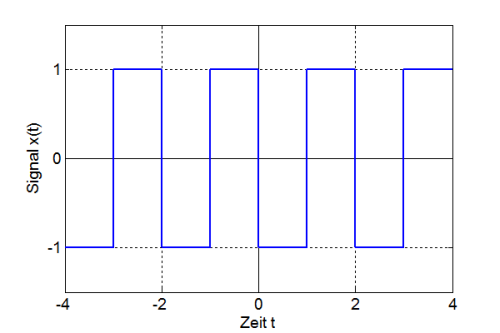
\includegraphics[width=0.45\textwidth]{img/rechteck}
      \caption{Quelle: Wikipedia}
\end{figure}

 \end{frame}

\begin{frame}
    \frametitle{Frequenz- und Skalenraummethoden}
\framesubtitle{}

\begin{block}{Beispiel}
\begin{align*}
Sf(t)=& \tfrac{4h}{\pi}\left[\sin \omega t+\tfrac{1}{3}\sin3 \omega t+\tfrac {1}{5}\sin5 \omega t+\tfrac{1}{7}\sin7 \omega t+ \cdots\right]\\
=& \tfrac{4h}{\pi} \sum_{k=1}^\infty \dfrac{ \sin\left( (2k-1)\omega t \right) }{2k-1} \\
& \omega = 2 \pi \cdot f
\end{align*}
\end{block}
\begin{figure}[htp]
      \centering
    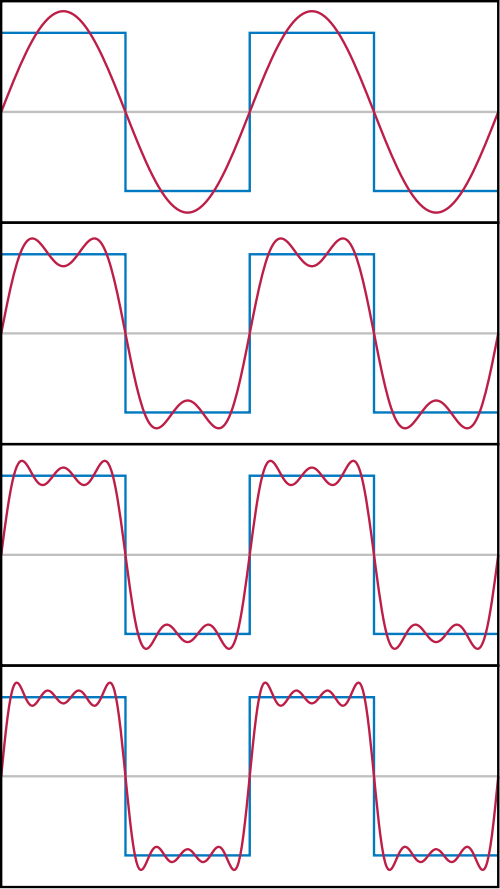
\includegraphics[width=0.15\textwidth]{img/fourier_example}
      \caption{Quelle: Wikipedia}
\end{figure}

 \end{frame}



\begin{frame}
    \frametitle{Frequenz- und Skalenraummethoden}
\framesubtitle{}

\begin{figure}[htp]
      \centering
    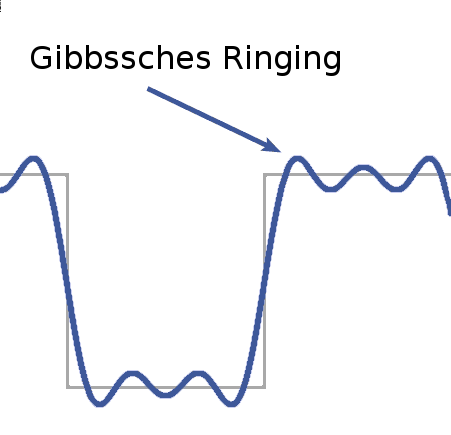
\includegraphics[width=0.35\textwidth]{img/Gibb}
      \caption{Quelle: Wikipedia}
\end{figure}

 \end{frame}



\begin{frame}
    \frametitle{Frequenz- und Skalenraummethoden}
\framesubtitle{}

\begin{block}{Fouriertransformation}
Sei $f: \mathbb{R}^n \to \mathbb{R}$ eine integrierbare Funktion. Die (kontinuierliche) Fourier-Transformierte ist definiert durch
\begin{align*}
\hat{ f}(y) = \frac{1}{\left(2\pi \right)^{n/2}} \int_{\mathbb{R}^n} f(x)\,e^{-i  <y, x>} \, d x,
\end{align*}
(Verallgemeinerung der Fourierkoeffizienten für nicht ganzzahlige Frequenzanteile).
\end{block}
\begin{block}{Schnelle Fouriertransformation}
Die Fouriertransformierte lässt sich approximativ und effizient auf dem Computer  berechnen:
\href{https://en.wikipedia.org/wiki/Fast_Fourier_transform}{LINK!}
\end{block}
 \end{frame}


\begin{frame}
    \frametitle{Frequenz- und Skalenraummethoden}
\framesubtitle{}

\begin{block}{Umkehrsatz}
Ist $f: \mathbb{R}^n  \to  \mathbb{R}$ und $\hat{ f}$ integrierbar, gilt
\begin{align*}
f(x) = \frac{1}{\left(2\pi \right)^{n/2}} \int_{\mathbb{R}^n}\hat{ f}(y) \,e^{i  <x, y>} \, d y,
\end{align*}
fast überall.
\end{block}
 \end{frame}


\begin{frame}
    \frametitle{Frequenz- und Skalenraummethoden}
\framesubtitle{}
\begin{block}{Nyquist-Shannon-Abtasttheorem}
Eine messbare Funktion $f: \mathbb{R} \to  \mathbb{R}$, deren Fouriertransformierte $\hat{f}$ außerhalb des intervals $(-b,b)$ verschwindet (bandbeschränkt), kann für jedes $T < \frac{\pi}{b}$ aus ihren Werten $f(kT), \; k \in \mathbb{Z}$ rekonstruiert werden, denn es gilt:
\begin{align*}
& f(x) = \sum_{-\infty}^{\infty} f(kT) \cdot sinc \biggl (\frac{\pi}{T}(x - kT) \biggr) \\
& sinc(x): = \frac{\sin x}{x}
\end{align*}
\end{block}
\begin{block}{Beweisidee}
Die Fouriertransformierte ist periodisch fortsetzbar, da bandbeschränkt. Daher existiert die Fourierreihe der Fouriertransformierten. Der Umkehrsatz angewendet auf diese Reihe liefert das Ergebnis.
\end{block}
 \end{frame}

\begin{frame}
    \frametitle{Frequenz- und Skalenraummethoden}
\framesubtitle{}

\begin{block}{Abtastrate}
Ein bandbeschränktes Signal mit höchster Frequenz $f = 2 \pi b$, kann  mit einer Abtastrate von mindestens $\frac{1}{2f}$ vollständig rekonstruiert werden. 
\end{block}
\begin{figure}[htp]
      \centering
    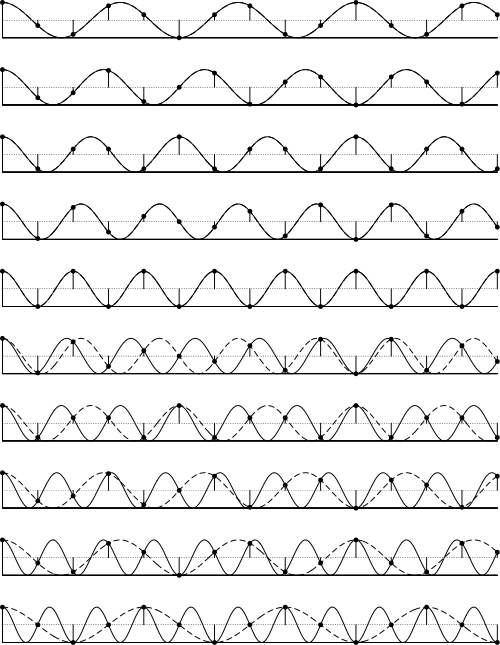
\includegraphics[width=0.35\textwidth]{img/Abtast}
      \caption{Quelle: Wikipedia}
\end{figure}

 \end{frame}

\begin{frame}
    \frametitle{Frequenz- und Skalenraummethoden}
\framesubtitle{}

\begin{block}{Alias Effekt}
Ist die Abtastfrequenz zu niedrig, kommt es zum sogenannten Alias Effekt.
\end{block}
\begin{figure}[htp]
      \centering
    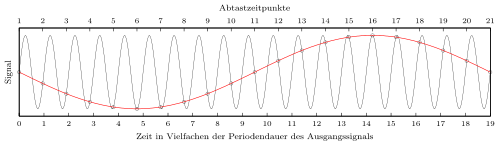
\includegraphics[width=0.65\textwidth]{img/Alias} \\ 
    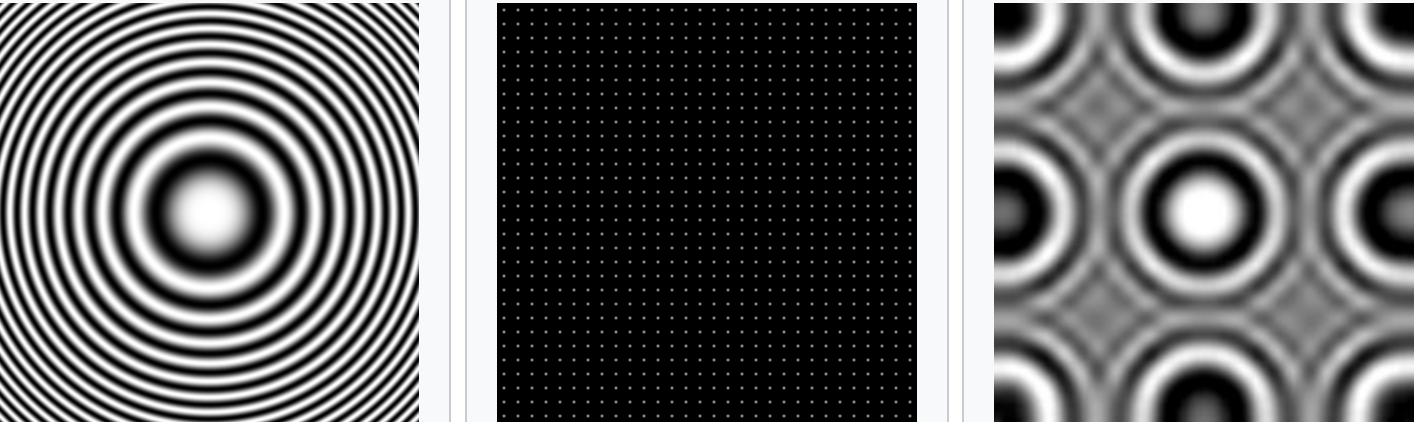
\includegraphics[width=0.65\textwidth]{img/Alias_img}
      \caption{Quelle: Wikipedia}
\end{figure}

 \end{frame}

\begin{frame}
    \frametitle{Frequenz- und Skalenraummethoden}
\framesubtitle{}

\begin{block}{Frequenz-Filter}
Gegeben ist eine Funktion $f$ und eine Filter-Funktion $g$. 
Die mit $g$ gefilterte Funktion erhält man durch  Rücktransformationen  der mit $g$ Multiplizierten Fouriertransformierten Funktion 
\begin{align*}
f_g := \frac{1}{\left(2\pi \right)^{n/2}} \int_{\mathbb{R}^n} g(y) \cdot \hat{ f}(y) \,e^{i  <x, y>} \, d y,
\end{align*}
\end{block}

 \end{frame}
\end{document}
